%%%%%%%%%%%%%%%%%%%%%%%%%%%%%%%%%%%%

\section{割合の信頼区間}

%%%%%%%%%%%%%%%%%%%%%%%%%%%%%%%%%%%%

\subsection{母集団パラメータの捕捉}

%%%%%%%%%%%%%%%%%%%%%%%%%%%%%%%%%%%%

\begin{frame}[shrink]
\frametitle{信頼区間}

\begin{itemize}

\item 母集団パラメータの妥当な値の範囲を\hl{信頼区間}と呼ぶ。

\item 標本統計量だけを使ってパラメータを推定することは、濁った湖で銛を使って魚を突こうとするようなものであり、信頼区間を使うことは網を使って魚を捕まえようとするようなものである。
$\:$ \\
$\:$ \\
\begin{columns}[c]
\column{0.25\textwidth}
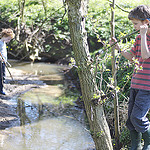
\includegraphics[width=\textwidth]{5-2_ci_prop/figures/spear}
\column{0.5\textwidth}
{\small
魚を見た場所に銛を投げても、たいていは外れてしまう。その辺りに網を投げれば、魚を捕まえる可能性が高い。
}
\column{0.25\textwidth}

\includegraphics[width=\textwidth]{5-2_ci_prop/figures/net}
\end{columns}
$\:$ \\
\item 点推定値を報告しても、正確な母集団パラメータには当たらないかもしれない。妥当な値の範囲を報告すれば、パラメータを捉える可能性が高くなる。

\end{itemize}

{\tiny 写真提供：Mark Fischer (http://www.flickr.com/photos/fischerfotos/7439791462) および Chris Penny (http://www.flickr.com/photos/clearlydived/7029109617) on Flickr.}

\end{frame}

%%%%%%%%%%%%%%%%%%%%%%%%%%%%%%%%%%%%

\subsection{95\%信頼区間の構築}

%%%%%%%%%%%%%%%%%%%%%%%%%%%%%%%%%%%%

\begin{frame}
\frametitle{Facebookによるユーザー興味分類}

\dq{多くの商業ウェブサイト（ソーシャルメディアプラットフォーム、ニュースサイト、オンライン小売業者など）はユーザーの行動データを収集し、ターゲットを絞ったコンテンツ、おすすめ、広告の配信に活用している。アルゴリズムによる分類システムがアメリカ人の実際の生活をどの程度反映しているかを理解するため、ピュー・リサーチはアメリカのFacebookユーザー850人の代表的な標本に対し、Facebookの「興味のあるもの」ページに表示されたカテゴリーが自分や自分の興味を正確に表しているかどうかを尋ねた。回答者の67\%が、表示されたカテゴリーは正確だと答えた。Facebookが自分の興味を正確に分類していると思うアメリカのFacebookユーザーの真の割合を推定せよ。}

\ct{\webURL{https://www.pewinternet.org/2019/01/16/facebook-algorithms-and-personal-data/}}

\end{frame}

%%%%%%%%%%%%%%%%%%%%%%%%%%%%%%%%%%%%

\begin{frame}
\frametitle{Facebookによるユーザー興味分類}

\[ \hat{p} = 0.67 \qquad n = 850 \]

おおよその95\%信頼区間は次のように定義される：
\[ \text{点推定値} \pm 1.96 \times SE \]

\vspace{-0.25cm}
\[ SE = \sqrt{\frac{p(1-p)}{n}} = \sqrt{\frac{0.67 \times 0.33}{850}} \approx 0.016 \]

\vspace{-0.25cm}
\begin{eqnarray*}
\hat{p} \pm 1.96 \times SE &=& 0.67 \pm 1.96 \times 0.016 \\
&=& (0.67 - 0.03, 0.67 + 0.03) \\
&=& (0.64, 0.70)
\end{eqnarray*}


\end{frame}

%%%%%%%%%%%%%%%%%%%%%%%%%%%%%%%%%%%

\begin{frame}
\frametitle{}

\pq{この信頼区間の正しい解釈はどれか？}

95\%の確信を持って言えることは：
\begin{enumerate}[(a)]
\item この標本のアメリカのFacebookユーザーの64\%から70\%が、Facebookは自分の興味を正確に分類していると思っている。
\solnMult{アメリカのFacebookユーザー全体の64\%から70\%が、Facebookは自分の興味を正確に分類していると思っている}
\item 無作為に選ばれたアメリカのFacebookユーザーの興味が正確に分類されている確率が64\%から70\%である。
\item アメリカのFacebookユーザーの95\%の興味が正確に分類されている確率が64\%から70\%である。
\end{enumerate}

\end{frame}

%%%%%%%%%%%%%%%%%%%%%%%%%%%%%%%%%%%

\begin{frame}
\frametitle{「95\%の確信」とはどういう意味か？}

\begin{itemize}

\item 多くの標本を抽出し、$\text{点推定値} \pm 1.96 \times SE$ という式を使って各標本から信頼区間を構築したとする。

\item すると、その区間の約95\%が真の母集団割合（$p$）を含むことになる。

\end{itemize}

\end{frame}

%%%%%%%%%%%%%%%%%%%%%%%%%%%%%%%%%%%

\begin{frame}
\frametitle{区間の幅}

\dq{母集団パラメータをより確実に捉えたい場合、すなわち信頼水準を高めたい場合、より広い区間を使うべきか、それとも狭い区間を使うべきか？}

\soln{より広い区間。}

$\:$ \\

\dq{より広い区間を使うことの欠点はあるか？}
\begin{center}

\includegraphics[width=0.9\textwidth]{5-2_ci_prop/figures/garfield}
\end{center}

\soln{区間が広すぎると、あまり有用な情報が得られないかもしれない。}

{\scriptsize 画像出典：http://web.as.uky.edu/statistics/users/earo227/misc/garfield\_weather.gif}

\end{frame}

%%%%%%%%%%%%%%%%%%%%%%%%%%%%%%%%%%%

\subsection{信頼水準の変更}

%%%%%%%%%%%%%%%%%%%%%%%%%%%%%%%%%%%

\begin{frame}
\frametitle{信頼水準の変更}

\[ \text{点推定値} \pm z^\star \times SE \]

\begin{itemize}

\item 信頼区間において、$z^\star \times SE$ を\hl{誤差の範囲（許容誤差）}と呼び、ある標本に対して、信頼水準が変わると許容誤差も変わる。

\item 信頼水準を変えるには、上の式の $z^\star$ を調整する必要がある。

\item 実際によく使われる信頼水準は90\%、95\%、98\%、99\%である。

\item 95\%信頼区間では、$z^\star = 1.96$ である。

\item ただし、標準正規（$z$）分布を使えば、任意の信頼水準に対応する適切な $z^\star$ を求めることができる。

\end{itemize}

\end{frame}

%%%%%%%%%%%%%%%%%%%%%%%%%%%%%%%%%%%%

\begin{frame}

\pq{98\%信頼区間を計算する際の適切な $z^\star$ はどのZ値か？}

\begin{multicols}{2}
\begin{enumerate}[(a)]
\item $Z = 2.05$
\item $Z = 1.96$
\solnMult{$Z = 2.33$}
\item $Z = -2.33$
\item $Z = -1.65$
\item[]
\end{enumerate}
\end{multicols}

\soln{
\begin{center}
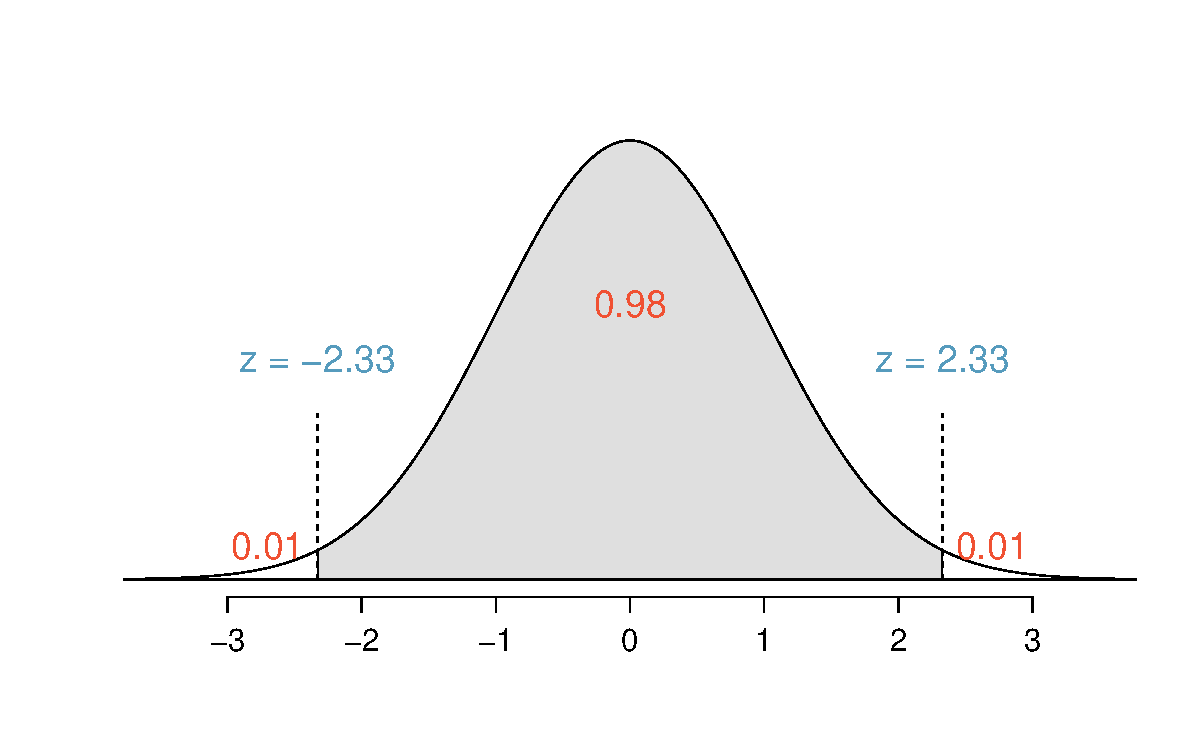
\includegraphics[width=0.7\textwidth]{5-2_ci_prop/figures/middle98/middle98}
\end{center}
}

\end{frame}

%%%%%%%%%%%%%%%%%%%%%%%%%%%%%%%%%%%

\subsection{信頼区間の解釈}

%%%%%%%%%%%%%%%%%%%%%%%%%%%%%%%%%%%

\begin{frame}
\frametitle{信頼区間の解釈}

信頼区間は…

\begin{itemize}

\item 常に母集団についてのものである

\item 確率の陳述ではない

\item 個々の観測値ではなく、母集団パラメータのみについてのものである

\item 基となる標本統計量が母集団パラメータの不偏推定量である場合にのみ信頼できる

\end{itemize}

\end{frame}

%%%%%%%%%%%%%%%%%%%%%%%%%%%%%%%%%%%
